\section{Luminaire Parameters}
For the calculations one type of luminaire has been chosen. From a wide range of outdoor luminaire procuders and distributors at the Czech market the luminaire Atos of the Schr\'{e}der company has been chosen.

\begin{figure}[htb]
  \centering
  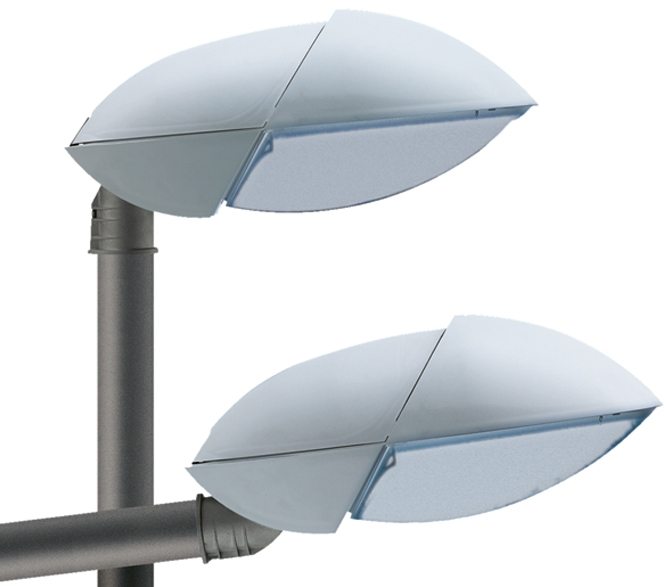
\includegraphics[width=0.7\columnwidth]{Atos}
  \caption{A photograph of the luminaire Atos}
  \label{fig:Atos}
\end{figure}

Atos luminaires are nowadays widely used for public outdoor lighting and can be fitted with light sources from 50~W to 150~W, making it suitable for road lighting of lower lighting classes, e.g. pedestrian zones, cycleways, emergency lanes etc.

The adjustment of luminous intensity distribution curves of Atos is achieved by changing the lamp position inside the luminaire with identical reflectors 1627~\cite{Schreder}. The luminaire Atos offers 12 different positions of the light source inside the luminaire (A1 to A4, B1 to B4 and C1 to C4), therefore 12 different luminous intensity distribution curves for each C-plane can be obtained.

\begin{figure}[htb]
  \centering
  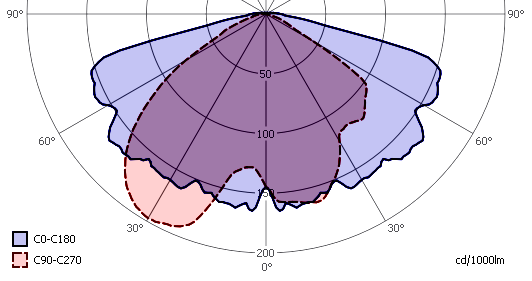
\includegraphics[width=\columnwidth]{70W_A1_v2}
  \caption{Luminous intensity distribution curves of ATOS/1627/SMOOTH POLYCARBONATE/SON-T 70/-17/100/10$^\circ$ for planes C0, C90, C180 and C270, exported from QLumEdit}
  \label{fig:lumIntDistr}
\end{figure}